\section{Methodology}

\subsection{Data}

\begin{equation}
    \frac{dL_\nu}{dM_{r}}=\epsilon_{\nu}(\rho,T)
\end{equation}

\begin{equation}
    \mathrm{Flux}=\frac{L}{4\pi r^2}
\end{equation}

\begin{figure}[H]
	\centering
	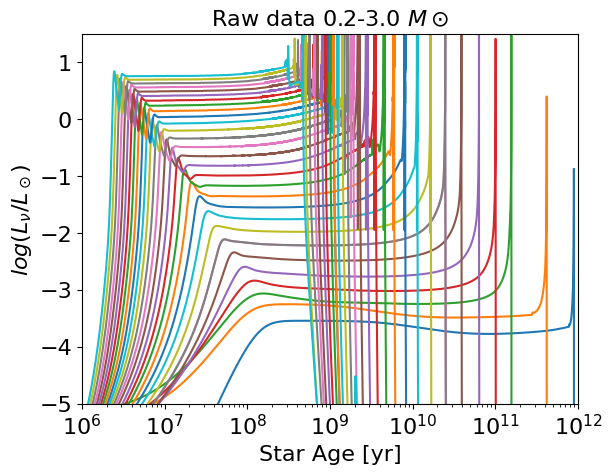
\includegraphics[width=\textwidth,height=\textheight]{assets/raw.png}
	\caption{Raw data $0.2-3.0 M\odot$.}
	\label{fig:raw}
\end{figure}


\subsection{Machine Learning}
Sci Kit Learn was used, specifically the Linear Regression module:
\begin{equation}
    y=\beta_{0}+\beta_{1}x_1+\beta_{2}x_2+\beta_{3}x_3+...+\beta_{n}x_n
\end{equation}
where 
$y$ is the independent variables, $\beta_0$ is the intercept, $\beta_{1}, \beta_{2}, \beta_{3},..., \beta_{n}$ is the coefficient. 

The basis of linear regression is the same as $y= mx+c$ but sklearn used more coefficients to predict the model. Linear regression estimate  coefficient such that the sum of error is very small ~  $10^{-4}$ (the tolerance adopted by sklearn). This method is also known as the least square method.

In this project the code will calculate the gradient B (written as J)  between the inputs which are the Masses and the Luminosity and the star ages.
\begin{equation}
    \mqty[
        m_{1}\\m_{2}\\m_{3}  
    ]
    J
    =
    \mqty[
        L_{11}&A_{11}&L_{12}&A_{12}&L_{13}&A_{13}\\
        L_{21}&A_{21}&L_{22}&A_{22}&L_{23}&A_{23}\\
        L_{31}&A_{31}&L_{32}&A_{32}&L_{33}&A_{33}
    ]
    \label{Eq:matrices}
\end{equation}
where $m$ is mass, $L$ is luminosity and $A$ is star age.
Equation\ref{Eq:matrices} is the representation on how the data was arranged in order to do the linear regression method. 

\begin{figure}[H]
    \centering

    \begin{tikzpicture}
        \node (A) at (-4,0) [draw, terminal] {Masses X($n\times 1$ )}; 
        \node (B) at (4,0) [draw, terminal] {Luminosity and Star Age Y($n \times m$)}; 
        \node (C) at (0,-2) [draw, process] {Zeroes Matrix J ($1\times m$)};
        \node (D) at (0,-4) [draw, process] {$\min_{J}||XJ-Y||^{2}$};
        \node (E) at (0,-6) [draw, process] {$J=(X^{T}X)^{-1}X^{T}Y$};
        \node (F) at (0,-8) [draw, process] {$X'J=Y'$};
        \node (G) at (0,-10) [draw, terminal] {OUTPUT};
        \draw[-{Latex}] (A) |- (C);
        \draw[-{Latex}] (B) |- (C);
        \draw[-{Latex}] (C) -- (D);
        \draw[-{Latex}] (D) -- (E);
        \draw[-{Latex}] (E) -- (F);
        \draw[-{Latex}] (F) -- (G);

    \end{tikzpicture}
    \caption{Flowchart of how the code does the linear regression.}
    \label{fig:flow}
\end{figure}

Figure~\ref{fig:flow} shows the flow of how the code does the linear regression. The code will take input Masses in the form of X$(n\times1)$ matrix and Luminosity and Star Age as Y$(n\times m)$ matrix. The code will then generate a zeros matrix J$(1\times m)$. The J will then be calculated using Equation\ref{Eq:leastsq} and then used in prediction.

\begin{equation}
    e=\sqrt{(x_p-x_g)^2+(y_p-y_g)^2}
    \label{Eq:er}
\end{equation}

Then using the Equation~\ref{Eq:er}, the error was calculated in term of the offset between predicted and grid data per mass.